\documentclass[11pt]{beamer}
\usetheme{Warsaw}
\usepackage[utf8]{inputenc}
\usepackage[french]{babel}
\usepackage[T1]{fontenc}
\usepackage{amsmath}
\usepackage{amsfonts}
\usepackage{amssymb}
\usepackage{graphicx}
\usepackage{array}
%\usepackage{easytable}
%\usepackage{tabularx}
\author{Sarah Kaddah}
\title{Results}
%\setbeamercovered{transparent} 
%\setbeamertemplate{navigation symbols}{} 
%\logo{} 
%\institute{} 
%\date{} 
%\subject{} 
\begin{document}

\begin{frame}
\titlepage
\end{frame}

%\begin{frame}
%\tableofcontents
%\end{frame}
%%%%%%%%%%%%%%%%%%%%%%%%%%%%%%%%%%%%%%%%%%%%%%%%%%%%%%%%%%%%%%%%%%%%%%%%%%%%%%%%%%%%%%%%%%%
\begin{frame}{Data}
\begin{center}
			% Tableau des données
			\medbreak						
			\begin{tabular}{|c|c|c|}
			\hline
			\begin{bf}Species\end{bf} & \begin{bf}\# of $\alpha$-sat.\end{bf} & \begin{bf}Sequencing method\end{bf}\\
			\hline
			\textit{Cercopithecus pogonias} & 112 902 & Ion torrent\\
			\hline
			\textit{Cercopithecus solatus} & 105 529 & Ion torrent\\
			\hline
			\textit{Chlorocebus sabaeus} & 29 842 & Illumina\\
			\hline
			\textit{Macaca fascicularis} & 39 893 & LS454\\
			\hline
			\textit{Macaca fascicularis} & 195 642 & Assembly\\
			\hline			
			\end{tabular}										
		\end{center}
\end{frame}
%%%%%%%%%%%%%%%%%%%%%%%%%%%%%%%%%%%%%%%%%%%%%%%%%%%%%%%%%%%%%%%%%%%%%%%%%%%%%%%%%%%%%%%%%%%
\begin{frame}{Comptage des familles et séquences}  
\begin{center}                    
	\begin{tabular}{|p{2cm}|p{1cm}|p{1cm}|p{1cm}|p{1cm}|p{1cm}|}
	\hline
	\begin{bf}\tiny{Species}\end{bf} & \begin{bf}\tiny{Nb of fam.}\end{bf} & \begin{bf}\tiny{Nb of small fam.}\end{bf} & \begin{bf}\tiny{Nb of big fam.}\end{bf} & \begin{bf} \tiny{\% seq. of seq. in small fam.}\end{bf} & \begin{bf} \tiny{\# of seq. in small fam.} \end{bf} \\
	\hline
	\textit{M. fascicularis 
	(SRA)}                   & 709 & 667 & 42 & 14.56 & 5807  \\
	\hline
	\textit{M. fascicularis 
	(Assembly)}              & ?   & ?   & ?  & ?     &?      \\
	\hline
	\textit{C. sabaeus}      & 338 & 294 & 44 & 10.89 & 3250  \\
	\hline
	\textit{C. pogonias}     & 169 & 155 & 14 & 1.63  & 1849  \\
	\hline
	\textit{C. solatus}      & 969 & 955 & 14 & 6.99  & 7372  \\
	\hline	
	\end{tabular}
\end{center}     
\end{frame}

%\begin{frame}{Comptage des familles et séquences} 
%\newcolumntype{M}[1]{>{\centering\arraybackslash}m{#1}}
%\begin{tabular}{|M{2cm}|p{1cm}|p{1cm}|M{1cm}|p{1cm}|p{1cm}|p{1cm}|}
%	\hline
%	\begin{bf}\tiny{Species}\end{bf} & \begin{bf}\tiny{Nb of fam.}\end{bf} & \begin{bf}\tiny{Nb of small fam.}\end{bf} & \begin{bf}\tiny{Nb of big fam.}\end{bf} & \begin{bf} \tiny{\% seq. of seq. in small fam.}\end{bf} & \begin{bf}\tiny{\% of seq. in big fam.} \end{bf} & \begin{bf} \tiny{\# of seq. in small fam.} \end{bf} \tabularnewline
%	\hline
%	\textit{M. fascicularis 
%	(SRA)}                   & 709 & 667 & 42 & 14.56 & 85.44 & 5807  \tabularnewline
%	\hline
%	\textit{M. fascicularis 
%	(Assembly)}              & ?   & ?   & ?  & ?     &?      & ?     \tabularnewline
%	\hline
%	\textit{C. sabaeus}      & 338 & 294 & 44 & 10.89 & 89.11 & 3250  \tabularnewline
%	\hline
%	\textit{C. pogonias}     & 169 & 155 & 14 & 1.63  & 98.36 & 1849  \tabularnewline
%	\hline
%	\textit{C. solatus}      & ?   & ?   & ?  & ?     &?      & ?     \tabularnewline
%	\hline	
%	\end{tabular}
%\end{frame}       

%%%                                               
\begin{frame}{Comptage des familles et séquences}{\textit{M. fascicularis}}
\begin{figure}
	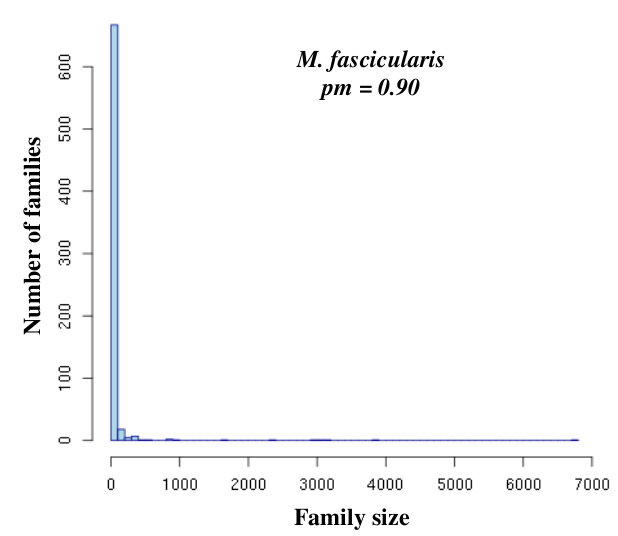
\includegraphics[width=0.8\textwidth]
		{img/Mf_hist_family_distribution_pm090.png}
	\end{figure}	  
\end{frame}
%%%%
\begin{frame}{Comptage des familles et séquences}{\textit{C. sabaeus}}
\begin{figure}
	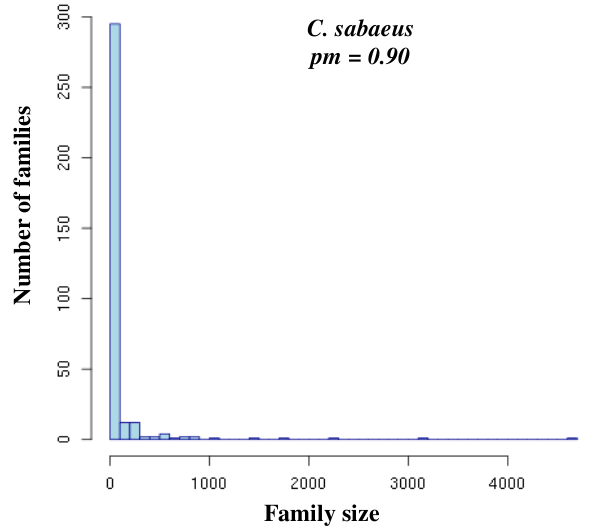
\includegraphics[width=0.8\textwidth]
		{img/Csa_hist_family_distribution_pm090.png}
	\end{figure}	  
\end{frame}
%%%%
\begin{frame}{Comptage des familles et séquences}{\textit{C. pogonias}}
\begin{figure}
	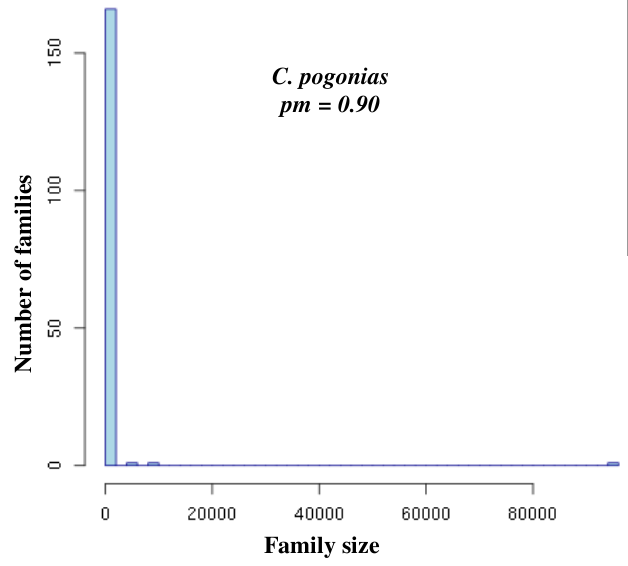
\includegraphics[width=0.8\textwidth]
		{img/Cp_hist_family_distribution_pm090.png}
	\end{figure}	  
\end{frame}
%%%%
\begin{frame}{Comptage des familles et séquences}{\textit{C. solatus}}
\begin{figure}
	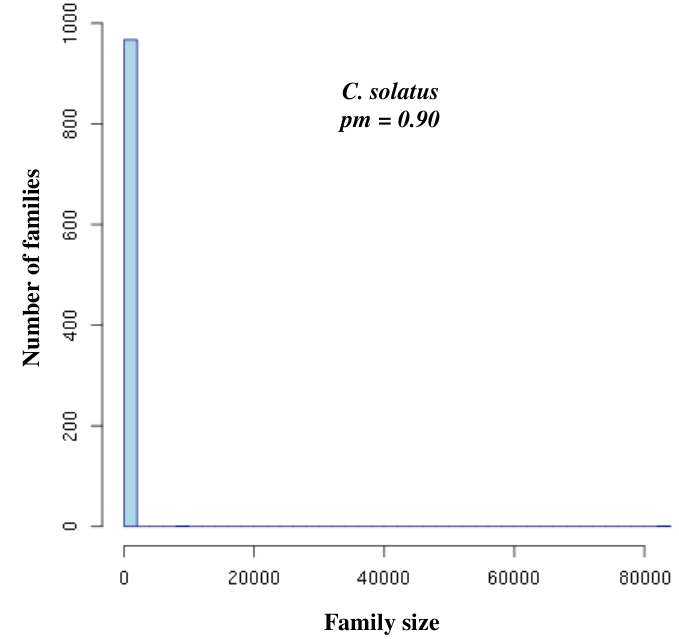
\includegraphics[width=0.8\textwidth]
		{img/Cso_hist_family_distribution_pm090.png}
	\end{figure}	  
\end{frame}
%%%%%%%%%%%%%%%%%%%%%%%%%%%%%%%%%%%%%%%%%%%%%%%%%%%%%%%%%%%%%%%%%%%%%%%%%%%%%%%%%%%%%%%%%%%
\begin{frame}{Binding sites}{\textit{M. fascicularis}}
	\begin{figure}
		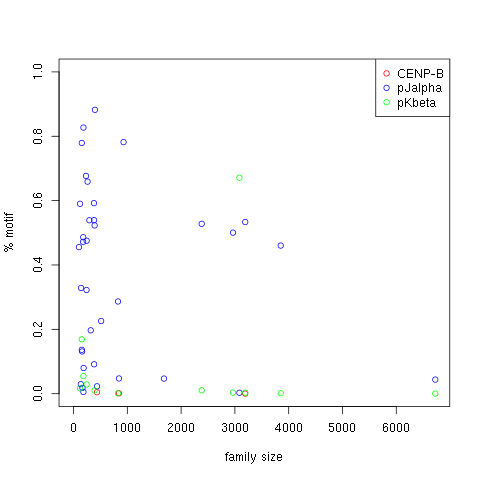
\includegraphics[width=0.75\textwidth]{img/Mf_motifs.png}
	\end{figure}	
\end{frame}

\begin{frame}{Binding sites}{\textit{C. sabaeus}}
\begin{center}
	\begin{figure}
		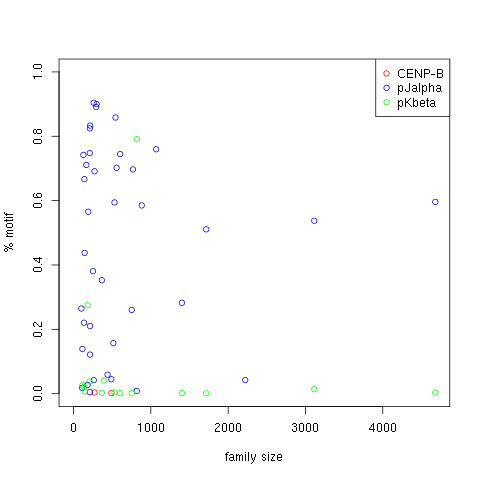
\includegraphics[width=0.75\textwidth]{img/Csa_motifs.png}
	\end{figure}	
\end{center}
\end{frame}

\begin{frame}{Binding sites}{\textit{C. pogonias}}
\begin{center}
	\begin{figure}
		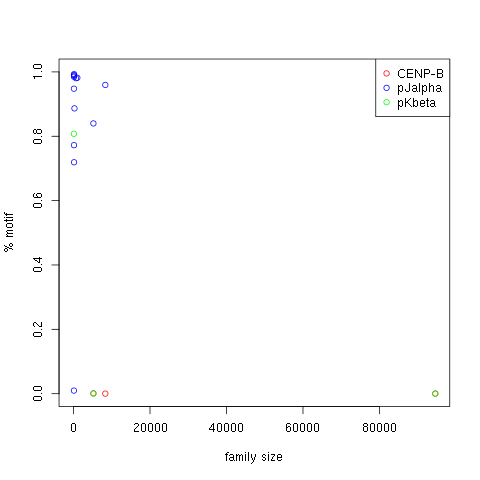
\includegraphics[width=0.75\textwidth]{img/Cp_motifs.png}
	\end{figure}	
\end{center}
\end{frame}

\begin{frame}{Binding sites}{\textit{C. solatus}}
\begin{center}
	\begin{figure}
		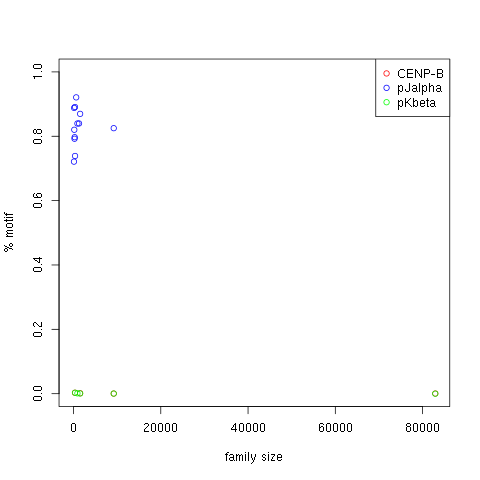
\includegraphics[width=0.75\textwidth]{img/Cso_motifs.png}
	\end{figure}	
\end{center}
\end{frame}
%%%%%%%%%%%%%%%%%%%%%%%%%%%%%%%%%%%%%%%%%%%%%%%%%%%%%%%%%%%%%%%%%%%%%%%%%%%%%%%%%%%%%%%%%%%
\begin{frame}{Similarity}{\textit{M. fascicularis}}
	\begin{figure}
		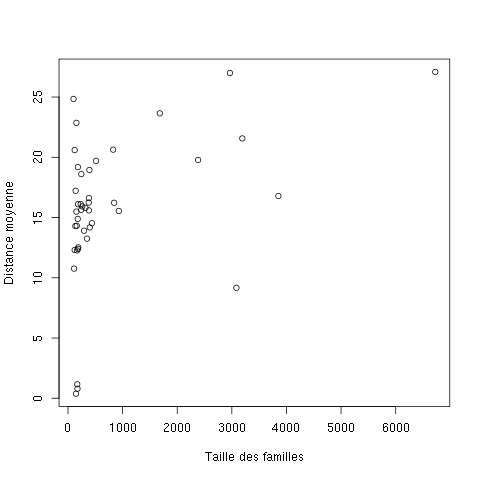
\includegraphics[width=0.75\textwidth]{img/Mf_similarity_090.png}
	\end{figure}	
\end{frame}

\begin{frame}{Similarity}{\textit{C. sabaeus}}
\begin{center}
	\begin{figure}
		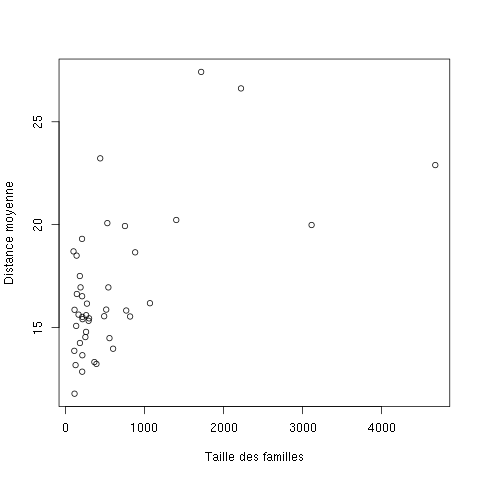
\includegraphics[width=0.75\textwidth]{img/Csa_similarity_090.png}
	\end{figure}	
\end{center}
\end{frame}

\begin{frame}{Similarity}{\textit{C. pogonias}}
\begin{center}
	\begin{figure}
		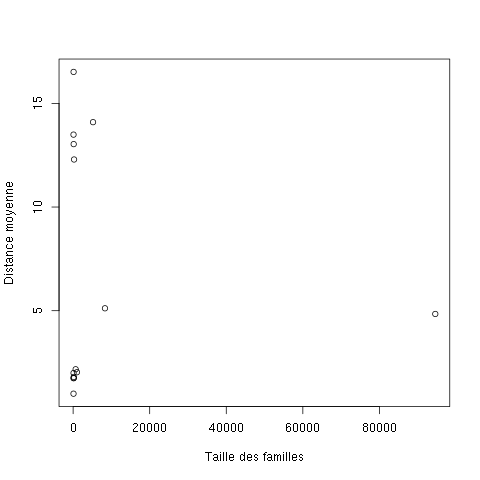
\includegraphics[width=0.75\textwidth]{img/Cp_similarity_090.png}
	\end{figure}	
\end{center}
\end{frame}

\begin{frame}{Similarity}{\textit{C. solatus}}
\begin{center}
	\begin{figure}
		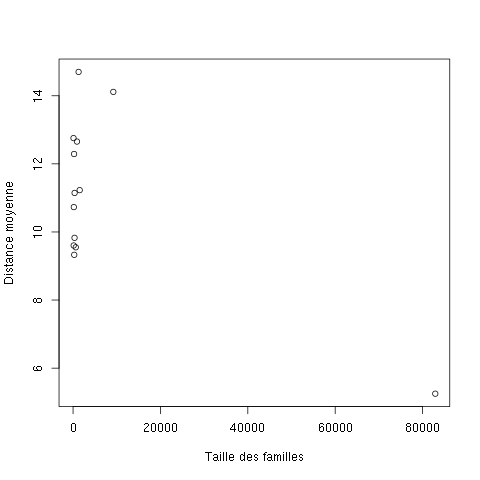
\includegraphics[width=0.75\textwidth]{img/Cso_similarity_090.png}
	\end{figure}	
\end{center}
\end{frame}
%%%%%%%%%%%%%%%%%%%%%%%%%%%%%%%%%%%%%%%%%%%%%%%%%%%%%%%%%%%%%%%%%%%%%%%%%%%%%%%%%%%%%%%%%%%
\begin{frame}{Calcul family size}
-\textit{Cercopithecus solatus}: \\
100 * 100 / 105 529 = 0.095\% = 0.00095\medbreak 

-\textit{Cercopithecus pogonias}:\\
100 * 100 / 112 902 = 0.089\% = 0.00089\medbreak 

-\textit{Macaca fascicularis} SRA:\\
100 * 100 / 39893 = 0.255\% = 0.0025\medbreak 

-\textit{Macaca fascicularis} Assembly:\\
100*100/195 642 = 0.051 = 0.00051\medbreak 

-\textit{Chlorocebus sabaeus}:\\
100 * 100 / 29842 = 0.34\% = 0.0034
\end{frame}

\end{document}